% Preamble
% --------
%
% amsmath : American Mathematical Society
% amssymb : American Mathematical Society symbols
% bm : Bold symbols in Math mode

\documentclass{article}
\usepackage{amsmath}
\usepackage{amssymb}
\usepackage{bm}
\usepackage{graphicx}
\usepackage{pgfplots}
\usepackage{gensymb}
\usepackage{blindtext}
\usepackage{titlesec}
\usepackage{tikz}
\usepackage{tikz-3dplot}
\pgfplotsset{compat=1.18}

\title{Notes about various mathematical topics.}
\author{Craig Sanders}
\date{ }

\setlength{\parindent}{0pt}


\begin{document}

\newpage

\maketitle

\newpage

\tableofcontents

\newpage

\listoffigures

% Document body

\newpage

\section{Introducting mathematical functions.}

\subsection{Numbers and their evolution.}

\noindent
\\
\textbullet \; The Natural numbers -- $\mathbb{N}$\\

A long time ago, humans counted using only the numbers $1$, $2$, $3$, and so on -- what we refer to nowadays
as the positive integers. The set of all these numbers is known as the Natural numbers, and is denoted by the
blackboard character $\mathbb{N}$.\\

\textbullet \; The Integer numbers -- $\mathbb{Z}$\\

Then gradually, over the course of time, first the concept of $0$ and then the negative integers, made their way
into the number system. The set of all these numbers -- when taken in conjunction with all of the numbers in 
$\mathbb{N}$, results in a new or expanded set of numbers called the Integers, and which is denoted by the
character $\mathbb{Z}$.\\

\textbullet \; The Rational numbers -- $\mathbb{Q}$\\

Then people started to do things like divide $1$ by $2$ to yield quotients, i.e. $1/2$. Numbers like this didn't
fit into the set represented by $\mathbb{Q}$, so $\mathbb{Q}$ was expanded even further to include numbers that
could be expressed as quotients or ratios. This set is denoted by the blackboard character $\mathbb{Q}$.\\

\textbullet \; The Real numbers -- $\mathbb{R}$\\

But then what about numbers like $\pi$, $e$, and so on -- numbers which are referred to an Irrational numbers,
because they can't be expressed as a ratio of two numbers.which can't be represented as quotients or fractions? In
order to accommodate numbers like these, $\mathbb{Q}$ was expanded again to include them. This set is denoted by
the blackboard character $\mathbb{R}$.\\

If you think of all the individual numbers which we might possibly use throughout the course of our everyday lives, $0$, $1$, $2$, 
$3$, $10$, $-100$, $\pi$, $0.000001$, $3817/245$ and so on; all of these numbers are encompassed by the set of 
Real numbers.\\

\textbullet \; The Complex numbers -- $\mathbb{C}$\\

Consider the result of $\sqrt{-1}$. Which of the aforementioned sets of numbers does the result live in? The answer
is that it doesn't live in any of them. Thus, to accommodate it, $\mathbb{R}$ was expanded once again, this time to
yield the set of Complex numbers. This set is denoted by the blackboard character $\mathbb{C}$.\\


\subsection{Numbers lines.}

We can think of every real number. i.e. every number which belongs to the set of Real numbers, as residing on an infinitely long straight line which stretches from
$-\infty$ to $+\infty$. We call this infinitely long straight line the real number line, and there is a place on this
line for any and all real numbers that we can think of.


\subsection{The amazing properties of $-1$.}

Consider the number $-1$ and what happens if we raise it to increasing integer powers.

\begin{align*}
(-1)^{0} &= 1  \;\;\; & \;\;\; (-1)^{1} &= -1 \\
(-1)^{2} &= 1  \;\;\; & \;\;\; (-1)^{3} &= -1 \\
(-1)^{4} &= 1  \;\;\; & \;\;\; (-1)^{5} &= -1
\end{align*}

\noindent
\\
\textbullet \; Integer valued function\\

Note how the resulting values alternate between $-1$ and $1$. If we were to represent these values as a function,
then it might look like the following;

\begin{equation}
\label{eqn:Square_wave}
f(x) = (-1)^{x} \;\; \vert \;\; x \in \mathbb{N} 
\end{equation} 

where the section that appears after the function definition, i.e.

\begin{equation*}
\vert \;\; x \in \mathbb{N}
\end{equation*}

can be thought of as a caveat which is to be applied to the function. This caveat is written in mathematical
nomenclature and can be interpreted as meaning ``such that (or where)  $x$ can only take on any integer number
value, i.e. any value from the set of integer numbers''.\\

Seeing as this caveat is applied to the function, the function will therefore only be defined when $x$ is equal
to an integer value. Graphing this function will result in a plot which looks as follows;

\begin{figure}[h!]
  \includegraphics[scale=0.75]{images/Square_wave_dots.png}
  \caption{This figure depicts the function $f(x) = (-1)^{x} \;\; \vert \;\; x \in \mathbb{N}$}
  \label{fig:Square_wave_dots}
\end{figure}


\noindent
\\
\textbullet \; Real valued function\\

If you don't like or don't feel comfortable with the integer number values caveat, then the function can be rewritten 
as follows, so that it makes use of real number values;

\begin{equation}
\label{eqn:Square_wave}
f(x) = (-1)^{\lfloor x\rfloor} \;\; \vert \;\; x \in \mathbb{R}
\end{equation}

where the $\lfloor\;\rfloor$ characters denote the mathematical floor function. Again, note that the function has a
caveat associated with it. The caveat is very similar to the previous one, except in this case it means 
``where  $x$ can only take any real number value''.\\

Plotting equation \ref{eqn:Square_wave} on a 2-dimensioanl Argand diagram results in the plot which is shown
in figure \ref{fig:Square_wave}.

\begin{figure}[h!]
  \includegraphics[scale=0.75]{images/Square_wave.png}
  \caption{This figure depicts the function $f(x) = (-1)^{\lfloor x\rfloor}$}
  \label{fig:Square_wave}
\end{figure}


\subsection{Imaginary numbers.}

There is however, a problem with this real number line and that is that it doesn't contain all the numbers!\\ 

Consider the number $-1$ and what will happen when we take the square root of it. The result will be $i$, where 
$i$ stands for ``imaginary number'' and unfortunately there is no place for this number -- or any multiples of it,
i.e. $i2$, $i100$, $-i707.87$ and so on, on the real number line. There is however, a place for $i$ on another
number line which we call the imaginary number line. We can also think
of this line as an infinitely long straight line, but instead of stretching from $-\infty$ to $+\infty$ like the real
number line, this one stretches from $-i\infty$ to $+i\infty$


\subsection{The slightly weird world of imaginary numbers.}

When compared with the real number line, the imaginary number line appears to exhibit some weird behaviour. 
In many ways it is just like the real number line, but in some ways it is not. If you add or subrtract multiple imaginary numbers together, you get another imaginary number. For example;

\begin{align*}
i + i &= i2 \\
i2 + i3 + i4 &= i9 \\
i50 - i100 &= -i50 
\end{align*}

This behaviour is just like the real number line. However, consider what happens when we start multiplying or dividing
imaginary numbers with each other.

\begin{align*}
i2 \times i3 &= -6 \\
i10 \div i5 &= 2 
\end{align*}

We can see here in these examples, that when an imaginary number is multiplied or divided by another imaginary
number, the result is a real number -- not another imaginary number. This is not what happens with real numbers.
With real numbers, multiplying or dividing one real number by another real number, yields a result that is
also a real number. That is, the types of the operands and the result in this case are all homogenous, i.e. 
they are all real numbers. This is an interesting observation which we will discuss in the next section. 

\subsection{Operation type transitivity.}

In the previous section, we discussed one of the differences between real and imaginary numbers. This difference
occurs when one of these numbers is multiplied with another number of the same type. I've devised a term for this
phenomenon because I can't find a pre-existing term which describes it; I call it ``operation type transivity'', and
it can take on the values of ``homogeneous'', ``heterogeneous'', or ``bigeneous''.\\

If a mathematical operator takes operands which are of a certain type -- say for example real numbers, and it
generates one or more values which are of this same type, then this function's operation type transivity is
referred to as being ``homogeneous''. This is excatly what happens when we multiply two real numbers together.\\

On the other hand, if a mathematical operator takes operands which are of another certain type -- say for example 
imaginary numbers this time, and it generates one or more values which are of a different type, then this function's 
operation type transivity is referred to as being ``heterogeneous''. This is exactly what happens when we multiply two
imaginary numbers together.\\

But what about operations which don't conform to concept of operation type homogeneity? We saw earlier that when 
two imaginary numbers are multiplied or divided with each other, the result is real. In this case, the operation
could be thought of as exhibiting ``operation type heterogeneity''.


\subsection{Multiplication and division of imaginary numbers.}

Why does multiplying or dividing two imaginmary numbers together result in heterogeneous operation types?
To help try and answer this, recall the definition of an imaginary number, that is;

\begin{equation*}
i = \sqrt{-1}
\end{equation*}

Therefore;

\begin{equation*}
i^{2} = -1
\end{equation*}

So for example, in the case where $i2 \times i3$, we essentially have;

\begin{align*}
i2 \times i3 &= (i \times 2) \times (i \times 3) \\
             &= i \times 2 \times i \times 3
\end{align*}

Re-arranging this yields;

\begin{align*}
i2 \times i3 &= (i \times i) \times (2 \times 3) \\
             &= i^{2} \times 6 \\
             &= -1 \times 6 \\
             &= -6
\end{align*}

Similarly, if we consider the division operation from above;

\begin{align*}
i10 \div i5 &= (i \times 10) / (i \times 5)
\end{align*}

Seeing as $i$ is common in both the numerator and the denominator, we can simply cancel them out with each other,
leaving a result of $2$.\\

What happens however, if we multiply or divide three imaginary numbers with each other? Consider the following
examples;

\begin{align*}
i2 \times \i3 \times i4 \\
(i24 \div i4) \div 3 
\end{align*}


\subsubsection{Loss of computing power.}

From the previous section, we can see that imaginary numbers start to lose some computational abilities when
compared to real numbers. A similar scenario occurs with quaternions, when compared to simple complex numbers. 


\subsection{Complex numbers.}

Consider the following mathematical expression;

\begin{equation*}
x + y
\end{equation*}

What is the deal with this expression when $x=1$ and $y=i1$? We can see that the result is comprised of two
parts; a real part $1$ and an imaginary part $i1$. Due to the fact that this number is comprised of two parts, it is
referred to as a ``complex number''. You might now be tempted to ask, which number line does this result reside on? The
answer to that question is that it resides on both the real and imaginary number lines. However, perhaps a better
answer is that
the result of this particular instance of the expression resides in a plane -- a complex plane to be more precise.
Let's elaborate a bit more in an attempt to try and explain exactly what this means. If we arrange the real and imaginary number
lines at right angles to each other, such that they intersect at 0, then we have what is known as a complex plane.
This value of $1 + i1$ can now be plotted on this complex plane.


\subsection{Denoting a function.}

Consider a function which is dependent on three separate and independent variables, \begin{math} x\end{math}, $y$ and 
\begin{math} z\end{math}. We can denote this function with the letter \begin{math} f \end{math} as follows;

\begin{equation*}
  f(x, y, z)
\end{equation*}

Note that within the declaration of this function, the three separate variables \begin{math} x\end{math}, 
\begin{math}y\end{math} and \begin{math} z\end{math}, are listed within parentheses.\\

This function could conceivably be used to model something like the colour represented by any point within a 
colour sphere; where \begin{math} x \end{math} could represent the forward and backward position within the
colour sphere, i.e. the yellow and blue axis, \begin{math} y \end{math} could represent the left and right position
within the colour sphere, i.e. the red and green axis, and \begin{math} z \end{math} could represent the up and down
position within the colour sphere, i.e. the black and white axis.

\newpage

\begin{figure}
  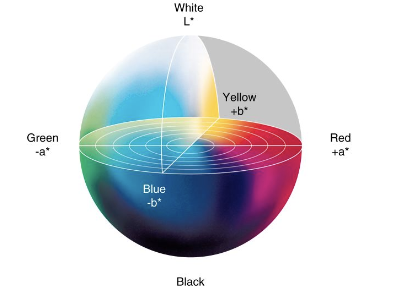
\includegraphics[scale=0.75]{images/Color_sphere.png}
  \caption{This figure depicts a 3-dimensional color sphere.}
  \label{fig:Color_sphere}
\end{figure}


\subsection{Defining a function.}

Let us now provide a definition or body for our function \begin{math} f \end{math}. We will see in the next section
why we have chosen this as the definition for our function -- that being, because it raises some interesting questions
about imaginary and complex numbers.

\begin{equation}
  f(x,y,z) = \sqrt{x} + \sqrt{y} + \sqrt{z}
\end{equation}

Note that the definition of the function is comprised of three distinct parts, $\sqrt{x}$, $\sqrt{y}$, and
$\sqrt{z}$, all of which are added together to yield the resulting value for the function. It is worth explicitly
mentioning that each of these three distinct parts is orthogonal to the other two, so they can't all simply be 
added together in such an easy manner as one might otherwise think!\\

Let's now put this function to one side for a moment, while we briefly discuss matrices and vectors, and how they might
help us with our definition of this function.


\subsection{Matrices.}

When presented in printed form, a matrix appears as a 2-dimensional mathematical construct
which is comprised of both rows and columns of values. The dimensions of any particular matrix can be described
as an \textit{m} x \textit{n} matrix -- where \textit{m} denotes the number or rows that make up the matrix, and
\textit{n} denotes the number of columns that make up the matrix. An example of a 2 x 3 
matrix, called $A$ in this case, is shown below;

\begin{equation*}
A = 
\begin{bmatrix}
2 & 8 & 5\\
7 & 4 & 1
\end{bmatrix}
\end{equation*}

where column 1 is comprised of the values 2 and 7, column 2 is comprised of the values 8 and 4, and column 3 is
comprised of the values 5 and 1. Similarly, row 1 is comprised of the values 2, 8, and 5, while row 2 is comprised
of the values 7, 4, and 1. It should be obvious now, that the reason we refer to this as a 2 x 3 matrix, is because
it is composed of 2 rows and 3 columns worth of values.\\

Consider the following function definition;

\begin{equation*}
f(x,y,z) = 2x + 3y + 4z
\end{equation*}

This function can be represented by the multiplication of two matrices as is shown below;

\begin{equation*}
f(x,y,z)= 
\begin{bmatrix}
2 & 3 & 4
\end{bmatrix}
\times
\begin{bmatrix}
x \\
y \\
z
\end{bmatrix}
\end{equation*}

 
\subsection{Vectors.}

Vectors are simply matrices which have a value of 1 for one of their dimensions. A benefit of vectors, is that 
they allow multi-part or multi-dimensional formula to be expressed in a more compact or succint manner. For example,
the function from earlier could be written in vector format as follows;

\begin{equation*}
f(x,y,z) = 
\begin{bmatrix}
\sqrt{x} & \sqrt{y} & \sqrt{z}
\end{bmatrix}
\end{equation*}

or, if a vertically oriented layout is preferred;

\begin{equation*}
f(x,y,z) = 
\begin{bmatrix}
\sqrt{x} \\
\sqrt{y} \\
\sqrt{z}
\end{bmatrix}
\end{equation*}


\subsection{Unit vectors.}

When a particular unit vector is used -- say for example
on a particular number line, then it denotes this number line as being orthogonal to all of the other number lines.
Since $\hat{\mathrm{\bm{i}}}$, $\hat{\mathrm{\bm{j}}}$, and $\hat{\mathrm{\bm{k}}}$ have now been applied
to the three parts of the function definition, we can now add them together using the mathematical addition operation,
i.e. $+$ without causing unnecessary confusion. This means that the three parts will add together in an orthogonal
sense to produce an overall 3-dimensioanl result.\\

Don't be confused by unit vectors. They can be thought in a sense as being a bit like direction readings when bush
walking. However, instead of being called north/south, east/west, or up/down, they are referred to as 
$\hat{\mathrm{\bm{i}}}$, $\hat{\mathrm{\bm{j}}}$, and $\hat{\mathrm{\bm{k}}}$. The image in \ref{fig:3d_axis} depicts what the three unit vectors look like, when 
they are overlaid onto a 3-dimensional Cartesian space which is comprised of x, y, and z axes.

\begin{figure}
  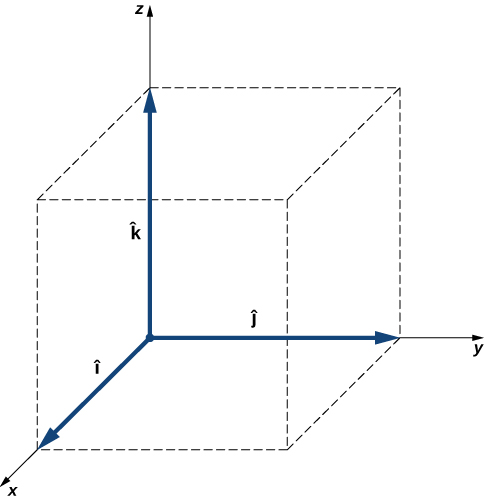
\includegraphics[scale=1.0]{images/3d_axis.jpg}
  \caption{This figure depicts a 3-dimensional Cartesian co-ordinate space $\mathbb{R}^3$ which is comprised
  of three orthogonal axes labelled x, y, and z. Overlaid in blue onto each of these three axes, are the three
  unit vectors, $\hat{\mathrm{\bm{i}}}$, $\hat{\mathrm{\bm{j}}}$, and $\hat{\mathrm{\bm{k}}}$.}
  \label{fig:3d_axis}
\end{figure}


\subsection{Complex vectors.}

Just as vectors can contain real numbers, they can also contain imaginary or complex numbers. For example;

\begin{equation*}
f(x,y,z) = 
\begin{bmatrix}
2 + i7 \\
5 + i3 \\
3 - i9
\end{bmatrix}
\end{equation*}

Could this function definition also be defined as;

\begin{equation*}
f(x,y,z) = \hat{\mathrm{\bm{i}}}(2 + i7) + \hat{\mathrm{\bm{j}}}(5 + i3) + \hat{\mathrm{\bm{k}}}(3 - i9)
\end{equation*}

This definition can potentially be thought of as being comprised of 6 dimensions. That is 3 dimensions in
the real space, i.e. $x$, $y$, and $z$, and a corresponding 3 dimensions in the imaginary domain. So how then, could
one go about plotting this function definition when it is comprised of so many dimensions?

\newpage
\section{Calculating the function.}

Earlier, we stated that we would assign the following definition to our function $f(x,y,z)$;

\begin{equation*}
  f(x,y,z) = \langle \sqrt{x}, \sqrt{y}, \sqrt{z} \rangle
\end{equation*}

Values of this function are simple enough to calculate when $x$, $y$, and $z$ are $\geq 0$, but what about when
these values are less than 0, for example;

\begin{align*}
  f(x,y,z) &= \langle \sqrt{-1}, \sqrt{-1}, \sqrt{-1} \rangle \\
           &= \hat{\mathrm{\bm{i}}}\sqrt{-1} + \hat{\mathrm{\bm{j}}}\sqrt{-1} + \hat{\mathrm{\bm{k}}}\sqrt{-1}
\end{align*}

According to the Wolfram Alpha website;

\begin{quote}
``Quaternions are a 4-dimensional number system that is an
extension of the field of complex numbers. A quaternion can be visualized as a rotation of vectors in three dimensions.''
\end{quote}

\subsection{Visualising the function by plotting it.}

\input{./subsections/square_root_x_y.tex}


\subsection{1-dimensional functions.}

1-dimensional functions don't rely upon any independent variables. For example, consider the following
mathematical expressions;

\begin{align*}
x^{2} &= 1 \\
x     &= 5 \\
y     &= \pi
\end{align*}

Let us take the first example and give it some further consideration. The first example can be re-arranged
as follows;

\begin{align*}
x &= \pm\sqrt{1} \\
  &= \pm1
\end{align*}

Plotting this simply results in two points on the 2-dimensional $x-y$ Argand diagram.

\begin{figure}
  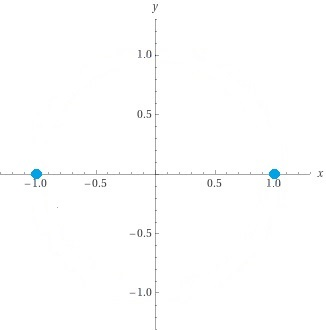
\includegraphics[scale=1.5]{images/Plus_and_minus_one.jpg}
  \caption{This figure depicts the result of plotting $x = \pm1$ on a 2-dimensional Argand diagram.}
  \label{fig:Plus_and_minus_one}
\end{figure}


\subsection{2-dimensional functions.}

2-dimensional functions rely upon a single independent variable. For example, consider the following mathematical
expressions;

\begin{align*}
f(x) &= x^{2} \\
f(x) &= x + 5 \\
y    &= x - \pi
\end{align*}

Note that the final example uses different nomenclature to the other two examples. The final example assigns the
result of the expression, i.e. $x - \pi$, to the dependent variable $y$.\\

Let us now expand the example which we singled out for further consideration in the previous section. We will
expand and rewrite this expression as follows;

\begin{equation}
x^{2} + y^{2} = 1
\end{equation}

This expression plots what is called a unit circle; that is a circle with radius 1 and which is centred on the origin 
of the $x-y$ plane. We can easily plot this expression on a 2-dimensional $x-y$ Argand diagram as is shown in figure .

\begin{figure}
  \begin{center}
  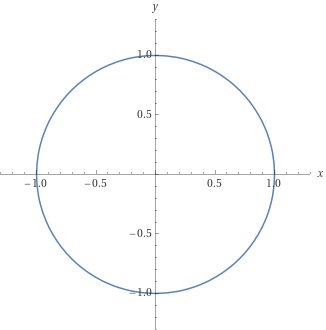
\includegraphics[scale=1.5]{images/Unit_circle.jpg}
  \end{center}
  \caption{This figure depicts a unit circle on a 2-dimensional Argand diagram.}
  \label{fig:Unit_circle}
\end{figure}


\subsection{3-dimensional functions.}

Let us now expand the example from the previous section, even further again. We will do this as follows;

\begin{equation}
x^{2} + y^{2} + z^{2} = 1
\end{equation}

This expression plots what is called a unit sphere; that is a 3-dimensional sphere with a radius of 1 and
which is centred on the origin of the $x-y-z$ space. An image of such a unit sphere is depicted in
\ref{fig:Unit_sphere}.

% \input{./subsections/sphere.tex}

\begin{figure}
  \begin{center}
  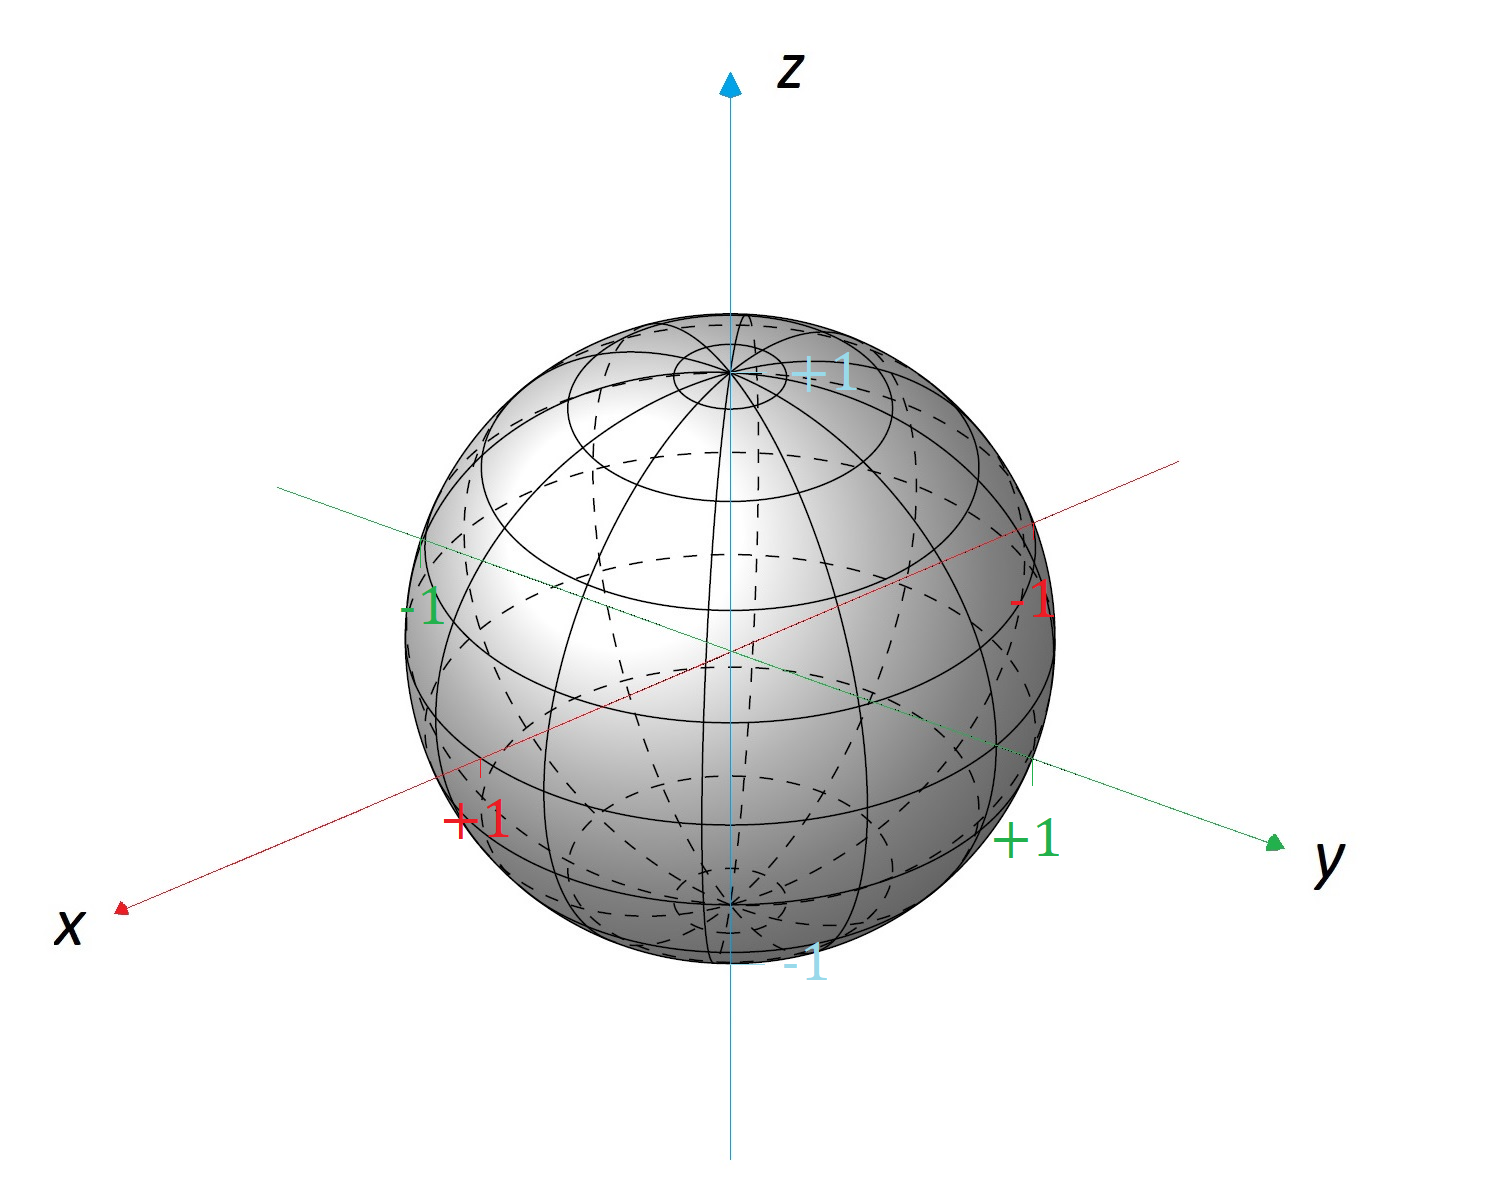
\includegraphics[scale=0.5]{images/Sphere_with_x_y_z_axes.png}
  \end{center}
  \caption{This figure depicts a unit sphere within a 3-dimensional co-oridnate axis system. Note that the $x$, $y$
           and $z$ axes have been coloured red, green and blue respectively. This has been done intentionally in an
           attempt to try and make them stand out against the unit sphere, which has been rendered in monochrome.}
  \label{fig:Unit_sphere}
\end{figure}


\subsection{4-dimensional functions.}

Let us once again expand upon the example from the previous section. This time we will add another independent
variable $a$, to the equation from the previous section, resulting in the following equation;

\begin{equation}
\label{eqn:Hyper-sphere_4d_1}
x^{2} + y^{2} + z^{2} + a^{2} = 1
\end{equation}

Note that this latest version of the equation is now comprised of four independent variables, that is $x$, $y$, $z$, 
and $a$. It is essentially the same equation that gave us the Unit sphere, but with the addition of one more
independent variable -- $a$. Furthermore, since the independent variable $a$ is also squared, the whole equation
can be thought of as describing a hyper-sphere. What is a hyper-sphere you might ask, it is simply a sphere that
is comprised of more than three dimensions.\\


\subsection{Limitations with visualising functions.}

The trouble with the hyper-sphere whose equation was just given above, is that it can't easily be visualised; afterall,
how can we visualise something in four dimensions? As we can see, equation \ref{eqn:Hyper-sphere_4d_1} is a
perfectly legitimate mathematical function -- it is just that we can't easily visualise it.


\section{The unit circle.}

Earlier, we saw how the following function generates a unit circle;

\begin{equation*}
x^2 + y^2 = 1
\end{equation*}

The appearance of this function is slightly odd, in the sense that both the $x$ and $y$ variables appear on
the same side of the equals sign. What if we were to re-arrange this function as follows;

\begin{align*}
x^2 + y^2 &= 1 \\
y^2 &= 1 - x^2 \\
y &= \sqrt{1 - x^{2}}
\end{align*}

Not sure this looks any better. What if we were to go back one step such that we have;

\begin{align*}
y^{2} &= 1 - x^{2}
\end{align*}

Re-arranging this gives;

\begin{equation*}
y^{2} = -x^{2} + 1
\end{equation*}

The right hand side of this equation is the function for an inverted parabola that has simply been shifted up by 1.
A plot of this is depicted in figure \ref{fig:Inverted_parabola}.

\begin{figure}
  \includegraphics[scale=1.0]{images/Inverted_parabola.png}
  \caption{This figure depicts a parabola which has been inverted and shifted up by one.}
  \label{fig:Inverted_parabola}
\end{figure}

Now consider what will happen if we take the square root of both sides of the equation. If we do this we get;

\begin{equation}
\label{eqn:Semi_circle}
y = \sqrt{-x^{2} + 1}
\end{equation}

The trouble with doing this is, that the square root operation only works when the number it is operating on is
$\geq 0$.\\

\begin{figure}
  \includegraphics[scale=0.8]{images/Square_root_of_inverted_parabola.png}
  \caption{This figure depicts the square root of a parabola which has been inverted and shifted up by one. That is,
  it depicts the function $f(x) = \sqrt{x^{2} + 1}$}
  \label{fig:Inverted_parabola}
\end{figure}

Okay, so now the function is only defined in the range $-1$ to $+1$. But what if we alter the function ever so
slightly so it becomes;

\begin{equation*}
y = \pm\sqrt{-x^{2} + 1}
\end{equation*}

The result of plotting this is shown in figure \ref{fig:Inverted_parabola}.

\begin{figure}
  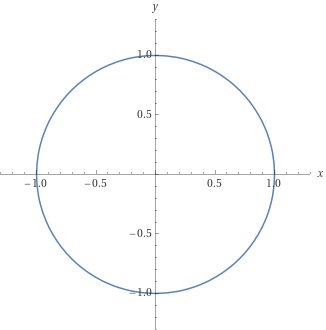
\includegraphics[scale=1.0]{images/Unit_circle.jpg}
  \caption{This figure depicts plus or minus the square root of a parabola which has been inverted and shifted
  up by one. That is, it depicts the function $f(x) = \pm\sqrt{x^{2} + 1}$}
  \label{fig:Unit_circle}
\end{figure}

Let's go back to equation \ref{eqn:Semi_circle} for a moment. Notice how this function ``fills out'' or ``pads out''
the inverted parabola which has been shifted up by one and is depicted in figure \ref{fig:Inverted_parabola}. This
all came about as another way to represent the equation;

\begin{equation*}
x^2 + y^2 = 1
\end{equation*}

But what would happen, if instead of squaring x and y, we raised them to the power of another even number -- say
four? That is;

\begin{equation*}
x^4 + y^4 = 1
\end{equation*}

We would get a plot which looks like this;





\end{document}